\begin{frame}
    - was ist cta?
    - was ist geplant?
    - was ist fertig?
    - womit können wir arbeiten?
    - status MC
    - was ist ctapipe?
    - wie soll es funktionieren? low-level-kram -> ? daten level? dl0,dl1,...?
    - status ctapipe
\end{frame}

\begin{frame}{column test}
    \begin{columns}[T] % align columns
        \begin{column}{.48\textwidth}
            \color{red}\rule{\linewidth}{4pt}
            \begin{enumerate}
                \item "Cherenkov Telescope Array"
                \item Proposed in 2005, currently in pre-production
                \item Two arrays of multiple telescopes (>100) instead of single telescopes
                \item Goals: Extend observable energy range(20GeV-300TeV), huge field of view()
                \item Status: First light on LST and Schwarzschildt-Couder-Telescope
            \end{enumerate}
        \end{column}%
        \hfill%
        \begin{column}{.48\textwidth}
            \color{blue}\rule{\linewidth}{4pt}
            \begin{figure}
                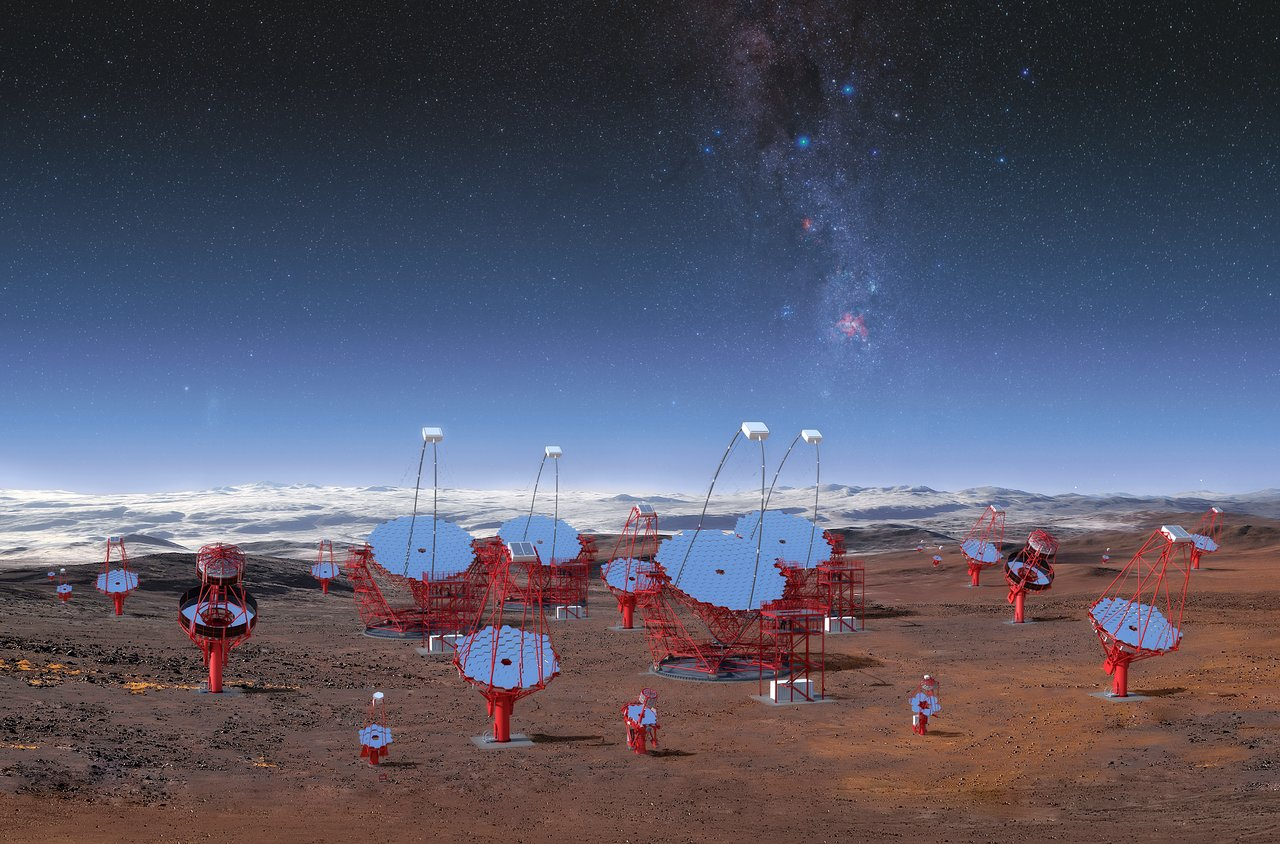
\includegraphics[width=\linewidth]{images/cta_telescopes.jpg}
                \caption{Visualization of the different telescope types. Credit: CTA/M-A. Besel/IAC (G.P. Diaz)/ESO}
            \end{figure}
        \end{column}%
    \end{columns}
\end{frame}


\begin{frame}{Expected sensitivity}
    \begin{figure}
        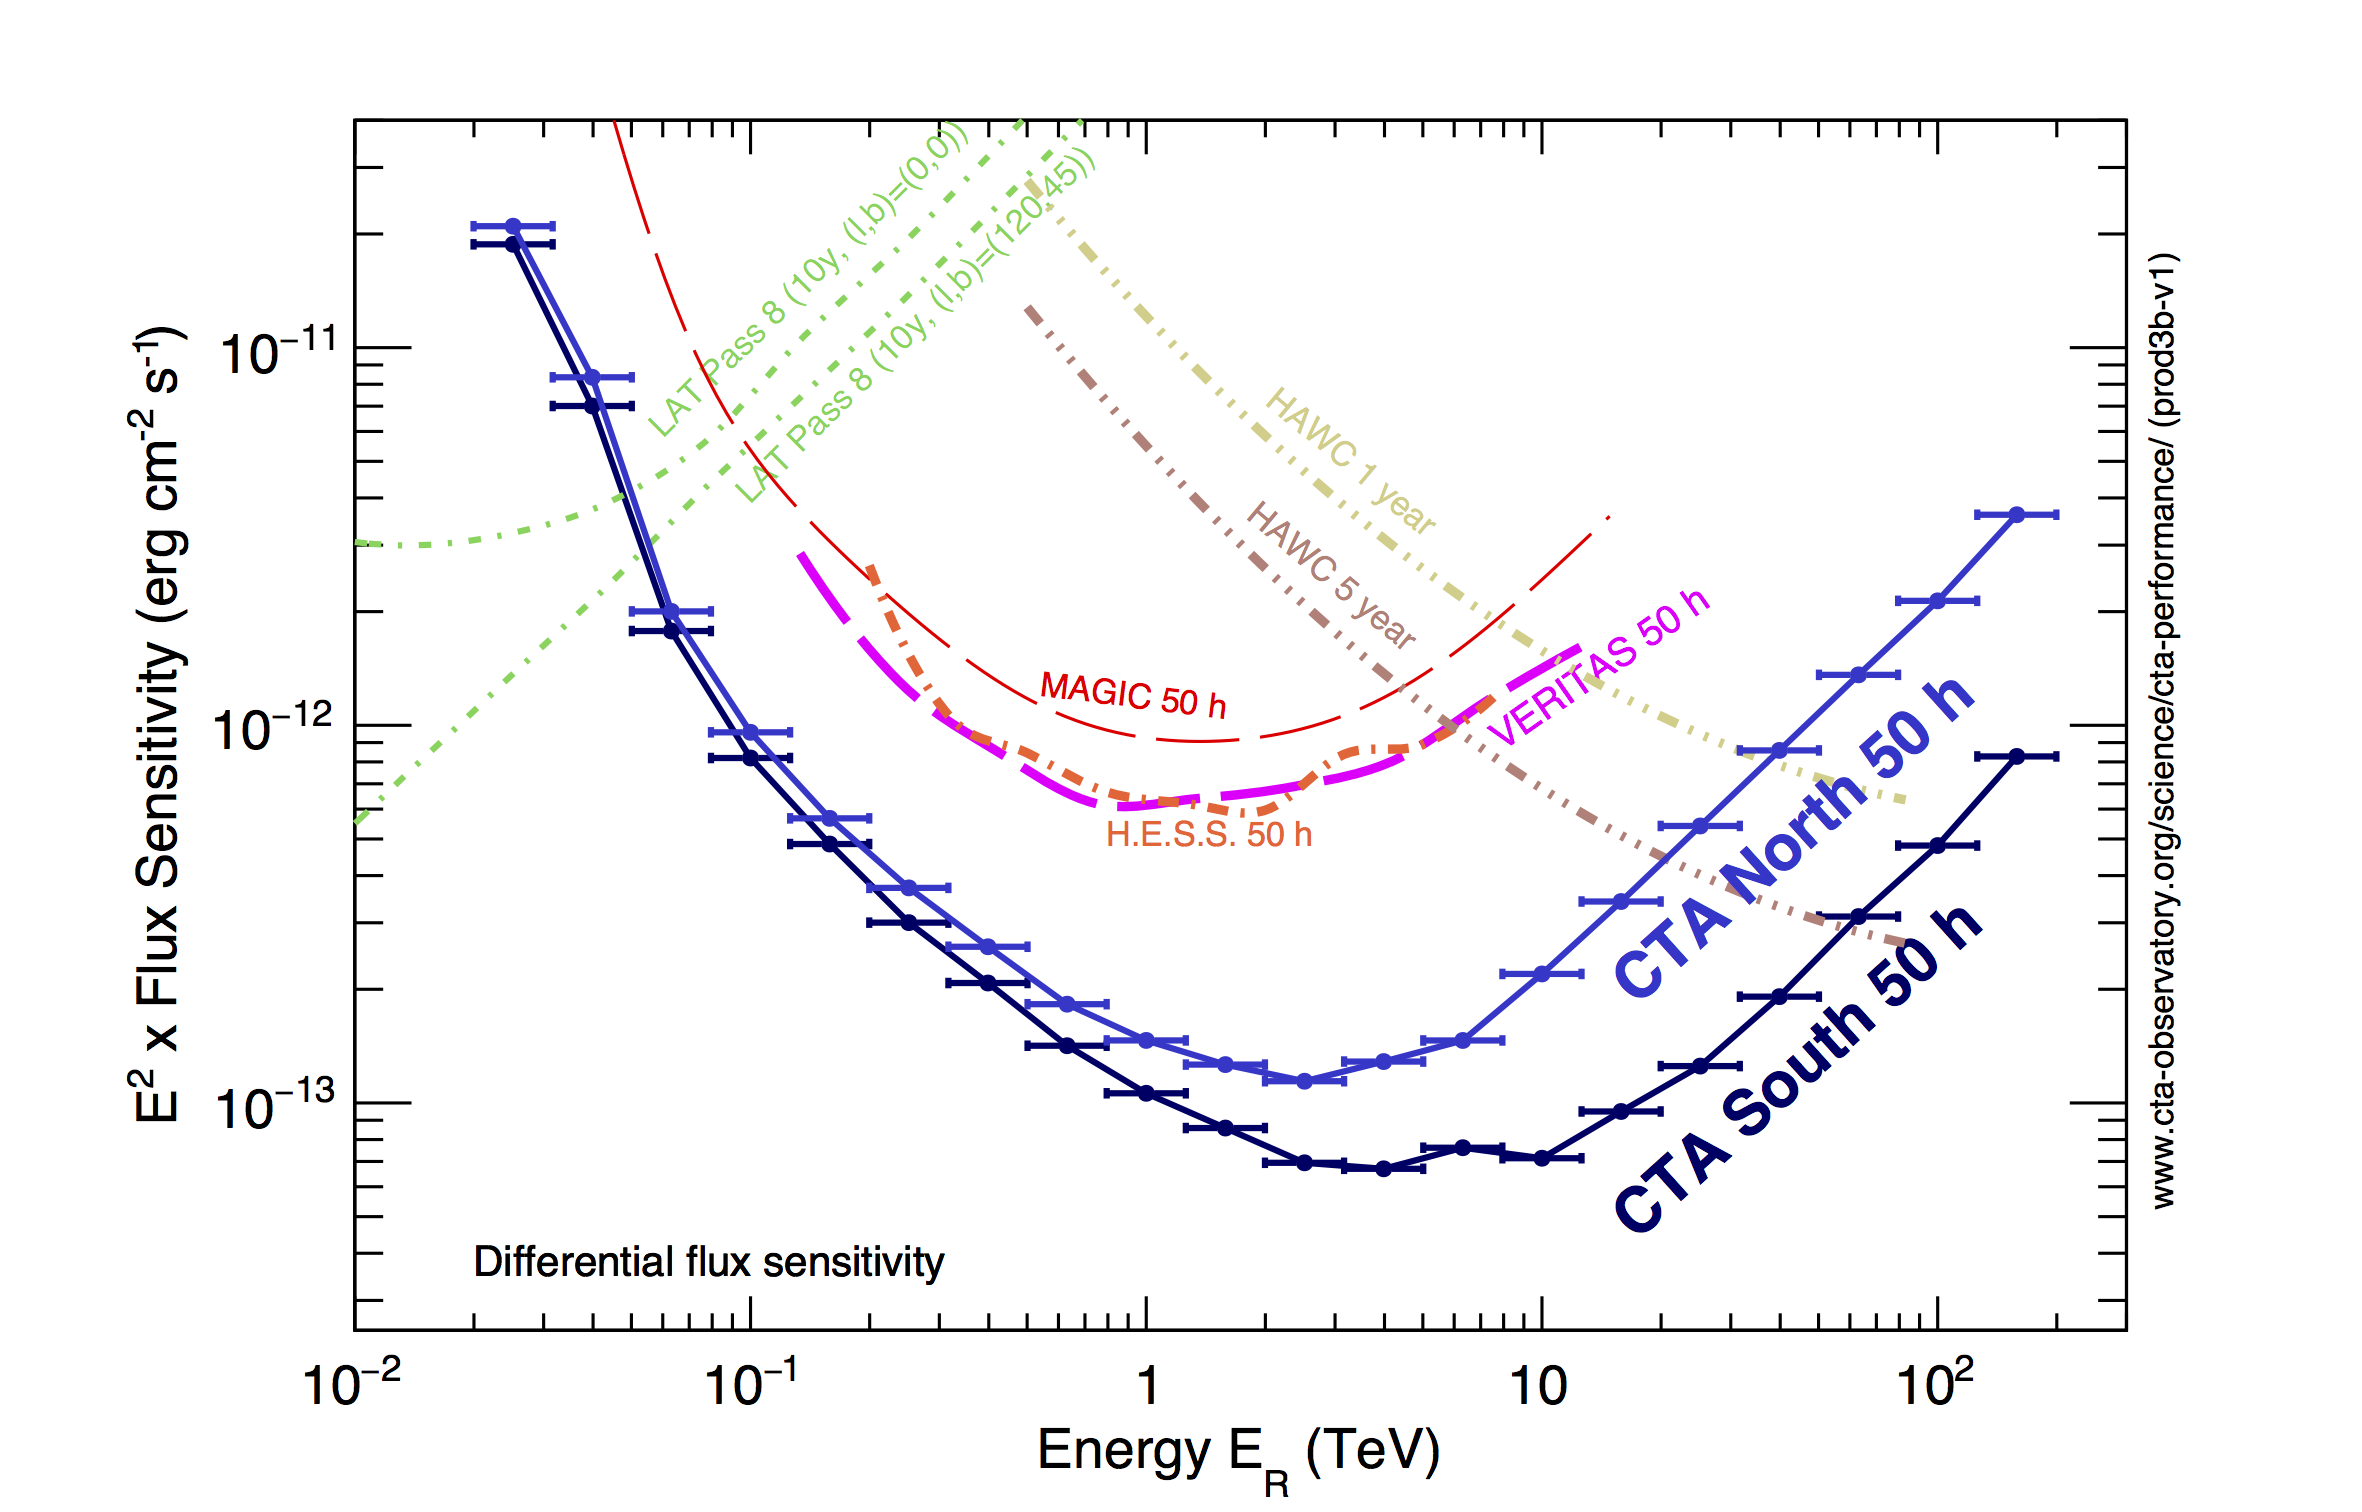
\includegraphics[width= 0.8\linewidth]{images/cta_sensitivity.png}
        \caption{Credit: CTA/M-A. Besel/IAC (G.P. Diaz)/ESO}
    \end{figure}

\end{frame}

\begin{frame}{ctapipe}
    \begin{enumerate}
        \item low level pipeline for cta data
        \item calibration, cleaning, hillas, ...
        \item in development, prototype
        \item python based
        \item ??
    \end{enumerate}
\end{frame}
